\chapter{Requirements and Development Options}

\section{Context}

In the previous chapter I presented the state of the art of smart shelves. 
To understand the context of the implementation presented throughout the remaining of this dissertation, I will contextualize its use case and background.

The smart shelve developed in this dissertation was primarily designed to integrate warehouse storage in Nespresso boutique stores.
Nespresso is a company owned by Nestlé Nespresso S. A., one operational unit of the Nestlé Group, dedicated to the retail and production of coffee capsules, coffee machines and related accessories.
Coffee arrives from different parts of the globe (Colombia, Brazil, Ethiopia, India, Indonesia, to say a few) through seaborne container, and reaches the factories by train.
The company has 3 manufacturing facilities producing coffee capsules in Switzerland, from where it dispatches products to supply chain centers.
Coffee machines are manufactured in East Europe.
Supply chain centers distribute the products to retail shops and boutique~\cite{PortugalRecebeCentro}.

With  the  growing  of  the  brand,  the  complexity  in  the logistics networks starts to compromise the management of the products down in the chain.
Namely, in boutique stores, the categorization and verification of new inventory, inspection of the arrived goods from the transportation company,  returns,  control  and  management  of  stocks, are all attended by manual labour. The manual labour is prone to errors and takes a lot of working time.

\subsection{Requirements}

The solution should be capable of being integrate with the logistics management software and services used by the company and trading partners.
The solution must be reliable and cheap to maintain.
The initial investment should also be the smallest possible.
The solution should be able to compose an inventory of the items in the shelve and provide means to store and query that data, preferably in a standardized manner following supply chain guidelines and practices.

(TODO: describe nespresso products, boxes, sleves)

\section{Solution}

The proposed solution is a system of smart shelving, where goods like coffee capsules, machines and accessories are stored. These goods would be \ac{rfid} tagged and integrated in an \ac{rfid}-enabled supply chain.
The structure storing the products contains \ac{rfid} antennas and readers that detect and read the tags attach to them. Readers will send real-time state of the products in stock to the software platform, which will contextualize the data, store it, and provide appropriate query interfaces to managing software systems.
In the future, the system could solve multiple issues and integrate multiple features like:

\begin{itemize}
    \item \textbf{Prevent stock-outs:} get timely replenishment and optimise in-store sales and management. Logistics companies deliver goods on time and according to delivery requirements generated automatically by a management system;
    \item \textbf{Reduce time and errors from manual labour:} counts, identification, misplacement and lost or stolen items;
    \item \textbf{Help customers:} find and engage with the products they want;
    \item \textbf{Control:} who removes or checks out valuable items;
    \item \textbf{Automatic information and management of stock:} the logistics lines automatically  transmits and receives stock information;
    \item \textbf{Smart physical storage:} automatic identification of goods in the warehouse/shelves, automatic matching of distribution requirements, improves the efficiency of goods storage;
    \item \textbf{Acquisition technology:} After the goods enter the collection area, the collection equipment automatically identifies multiple items by collecting \ac{rfid} tags, thereby efficiently completing the goods in and out of the warehouse, ensuring whether the physical and  distribution  requirements are consistent, and improving the efficiency of goods distribution;
    \item \textbf{Real-time:} master the distribution of all goods in real time, accurately grasp the inventory situation, optimize the inventory, and grasp the status and changes of the warehouse environment in real time;
    \item Handle registration and verification of arriving stock and manage in real time warehouse products;
    \item Real-time  management  of fall the  products, machine learning predictions and control of the product flow
\end{itemize}

In the design and planning of this solution, there were two very different contexts considered: the development of a real product, ready for the envisioned environment, where costs, implementation and architecture are well thought in order to achieve a stable and commercially appealing product; and a generic prototype implementation showing a working vision of what the real product would be like.

In the remaining of this chapter I will address the real product context, discussing and presenting multiple development options. In the last section~\ref{sec:ourchoice}, I will focus on the prototype solution proposal, which will focus on implementing the functional blocks required to the real product implementation, which will presented in dept in chapter~\ref{sec:systemdevelopment}.

\section{\acs{rfid} Technology}

It was clear, early in this work, that the \ac{rfid} technology which would be used was \ac{uhf}. 
\ac{uhf} is the most reasonable choice in this context: it has the reading distance requirements necessary for the solution envisioned; it provides the cheapest and most performant tags, with promises of even cheaper, more robust and efficient in the future; and most important, it is the \ac{rf} technology used in \ac{gen2} tags and \ac{scm} systems deployed around the globe. 
The integration in logistics and supply chain systems, would not make sense otherwise to diverge from the well established implementations.
With this, there is no further critical incentive to opt for other \ac{rfid} technology other than \ac{uhf} \ac{rfid}.

\section{Readers}

\subsection{Market Offer}

Choosing a reader is a complex subject. The market of RAIN \ac{rfid} \ac{gen2} compatible readers is extensive, but not very divergent in implementation, in that most readers are based on the same \ac{epc} Class 1 \ac{gen2} \ac{ic} chips.

From what I could find, currently, the available \ac{epc} Class 1 \ac{gen2} reader chips available on the market are listed on table~\ref{tab:readerchips}.
The biggest market leader is Impinj, which commercializes their own readers and development kits with their Indy reader chips~\cite{RAINRFIDReader} for most of commercial readers available on the market (e.g.\ CAEN RFID and Jadak ThingMagic modules~\cite{RAINRFIDPartner}).
There are other players in the \ac{epc} Class 1 \ac{gen2} reader chip manufacturer. 
STMicroelectronics acquired Austriamicrosystems' \ac{nfc} and \ac{rfid} reader assets in 2016~\cite{PressRelease}. Austriamicrosystems provided, the now discontinued, \texttt{AS3990} (i.g.\ \texttt{ST25RU3991}), \texttt{AS3990} (i.g.\ \texttt{ST25RU3992}) and \texttt{AS3980} (i.g.\ \texttt{ST25RU9080}) used by academics to create \acs{diy} cheap \ac{epc} Class 1 \ac{gen2} readers~\cite{tangDesignUHFRFID2010a, leiDesignHandheldUHF2011, liDesignRadioFrequency2011}. Currently STMicroelectronics
commercializes their \texttt{ST25RU3993} chip~\cite{ST25RU3993}. This chip is used in their evaluation boards and in few commercial readers~\cite{UHFMidRange}.
There are also companies selling SMD \ac{epc} Class 1 \ac{gen2} reader/writer modules, namely Nordic, with the ID NUR~\cite{NURModulesNordic}, and ThingMagic with the M6e, Micro and Nano~\cite{ThingMagicRFID}.

\begin{table}
    \centering
    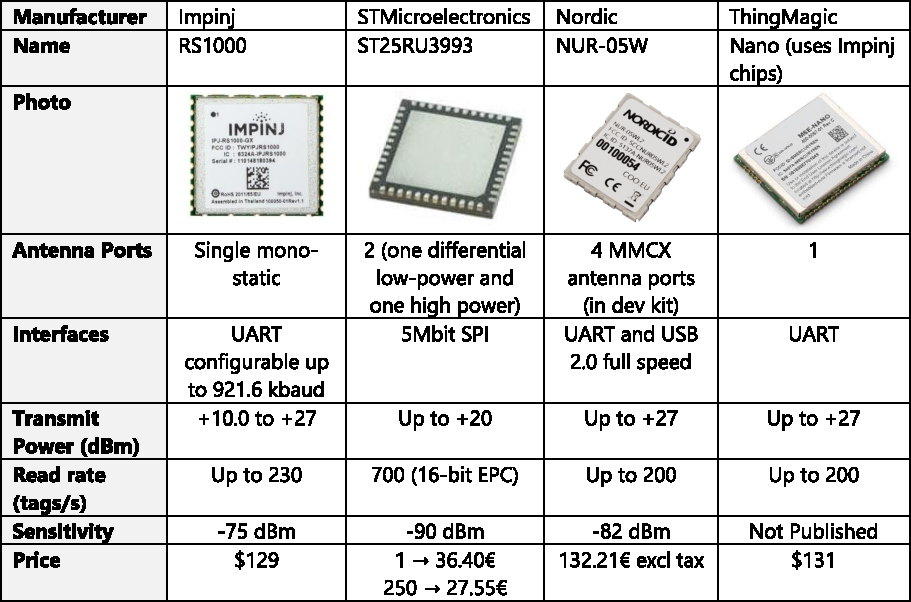
\includegraphics[width=\linewidth]{./figs/02-state-of-the-art/table_chipreaders.pdf}
    \caption[Available \ac{epc} Class 1 \ac{gen2} reader chips and SMD modules on the market]{Available \ac{epc} Class 1 \ac{gen2} reader chips and SMD modules on the market. Information and prices gathered from respective datasheets, AtlasRFIDstore~\cite{AtlasRFIDstoreBuyRFID} and Mouser~\cite{DistribuidorComponentesEletronicos}.}
    \label{tab:readerchips}
\end{table}

Regarding commercially available readers, there is an extensive variety of solutions, to many to discuss in this dissertation. A overview of established, widely deployed readers can be seen in table~\ref{tab:readercommercialsolutions}.
Alien Technology, has been commercializing their on \ac{rfid} readers~\cite{AlienTechnologyReaders} for years, having an well established client base. Impinj and Zebra have also been on the market, being well established \ac{epc} Class 1 \ac{gen2} reader manufacturers.

\begin{table}
    \centering
    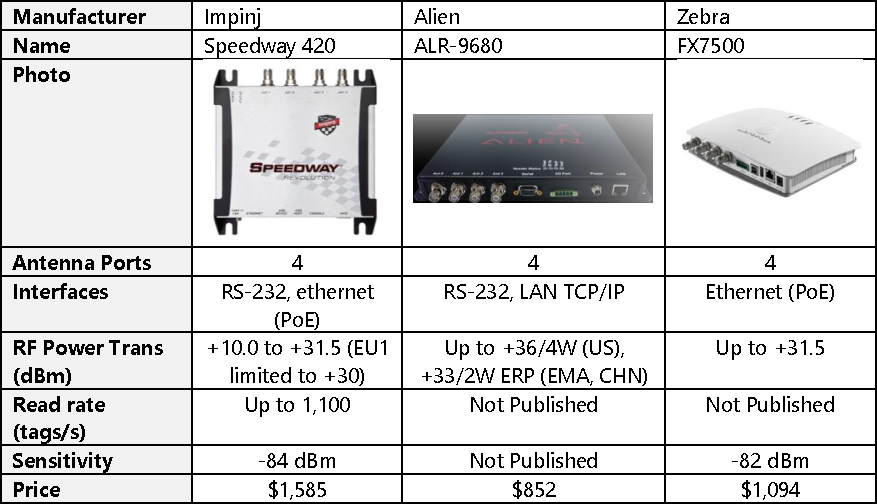
\includegraphics[width=\linewidth]{./figs/02-state-of-the-art/table_commercialreaders.pdf}
    \caption[\ac{epc} Class 1 \ac{gen2} compatible readers well established on the market]{\ac{epc} Class 1 \ac{gen2} compatible readers well established on the market. Information and prices gathered from respective datasheets and AtlasRFIDstore~\cite{AtlasRFIDstoreBuyRFID}.}
    \label{tab:readercommercialsolutions}
\end{table}

\subsection{Considerations}

Buy a commercial reader or make one?
The response is deeply dependent on company long term plans, namely, in the balance between \ac{rnd} cost and long term benefits. Compromises in engineering work have to be clearly balanced with the company needs and requirements. If the \ac{rfid} implementation plans extend deeply into the organization - points of sale, distribution centers, warehouses and manufacturing - making a custom reader solution might not be a total nonsense when evaluating cost margins and requirements. For companies like Walmart and big retailers, the investment in custom hardware definitely makes sense.

Commercial readers tend to be very expensive. They are usually designed for generic applications, providing incredible reading distances, astonishing number of tag reads per second, and multiple other features to please every client and fit every application.
This makes them rather expensive and excessive for applications like smart shelves.

Smart shelves, in most design approaches, do not require high transmission power nor high tags reads per second. Designs usually take advantage of \ac{rf} splitters and multiplexers to connect multiple antennas. They could also take advantage of Wifi, LTE and PoE capabilities, over the traditional communication interfaces like the serial port.

Said so, there are two paths which can be followed: development of a custom reader~\footnote{When I address the development of custom readers, I do not specify how, as it can be done through consulting companies or in house. In this dissertation I only approach development considerations and not how those are translated to engineering work} or the use of a commercial one. 
Custom designs for smart shelves can be much cheaper: less features translate to lower requirements in hardware; lower power transmission allows the use of cheaper \ac{rf} amplifiers (commercial readers can read up to $10m$, depending on implementations, might only be required reads up to $1m$); low requirements of reads speeds allow for cheaper \ac{epc} Class 1 \ac{gen2} SMD or chip solutions like handheld \ac{gen2} \acs{ic}.
On top of being cheaper, custom readers allow developers to implement features otherwise nonexistent. Many readers provide interfaces mainly through Java and C\# SDKs, open standards like \ac{llrp} are usually provided only in few high-end commercial readers. The stagnant condition of commercial readers do not keep up with new \ac{iot} and \ac{it} technologies, which have showed to be incredible powerful, mainly in the distributed computing area, and dismissed in favor of legacy technologies.
Custom readers can also integrate middleware capabilities (i.g.\ ``smart readers'' conceptualized by the \emph{EPCGlobal Architecture Framework}), and event capture application features, allowing a deprecation of discrete middleware and capture applications.
On the other hand, the development of such readers is \ac{rnd} intensive. For small and medium companies, such option is not remotely reasonable. Even for big companies, this kind of project would certainly be approached by consulting companies, since they are not at all within the expertise of most \ac{scm} and retailers.

\section{Antennas}

The discussion between custom and commercial readers made previously, can also be transposed to the selection of antennas. In certain conditions, the development of custom solutions can present good incentives.

Smart shelves, depending on implementations, require mainly antenna designs suitable for the \emph{near-field} region.
The market offers generic high performance antennas for most applications. These antennas also tend to be expensive, due to the strong requirements in reading distances. 

In the section~\ref{sec:academicsolutions}, I cited numerous implementations of of \emph{near-field} \ac{uhf} \ac{rfid} antennas, intended to be used in smart shelves and similar purposes, by the academic personnel. Many of these are simple and much cheaper than commercial alternatives, with performance suitable to be integrated in smart shelve systems. 

The approach taken in antenna selection, similarly to reader selection, depends on company approach to such endeavor. 
In table~\ref{tab:antennasolutions} presents a few compact commercial antennas considered for the implementation of this dissertation.

\begin{table}
    \centering
    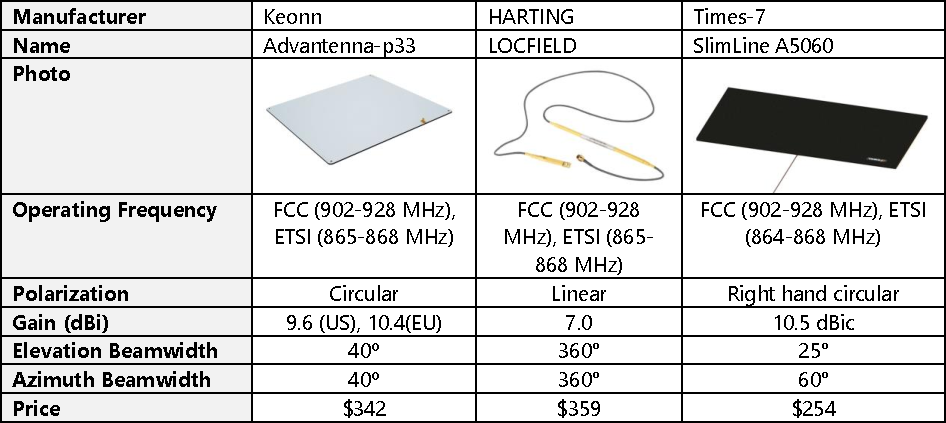
\includegraphics[width=\linewidth]{./figs/02-state-of-the-art/table_antennas.pdf}
    \caption[A few \ac{uhf} \ac{rfid} compact antennas available on the market]{A few \ac{uhf} \ac{rfid} compact antennas available on the market. Information and prices gathered from respective datasheets and AtlasRFIDstore~\cite{AtlasRFIDstoreBuyRFID}.}
    \label{tab:antennasolutions}
\end{table}

\section{Positioning}

Smart shelves can be implemented and designed taking different approaches (e.g.\ regarding number of antennas, their position and power transmitted).
D’Alessandro, in his PhD thesis~\cite{dalessandroRFIDBasedSmartShelving2012}, makes a good overview and evaluation of few possible combinations, which I used to elaborate the discussion in this section.
Following I will present a few architectural designs for \ac{uhf} \ac{rfid}-enabled smart shelves, how they differ, and discussed implementation considerations.

The first design, in figure~\ref{fig:position1}, is the simplest of all, a reader and one antenna. The figure shows a top view of a shelve with an external antenna, radiating it at an angle. Variations of this design can be found in retail stores with ceiling antennas pointing to shelves.
The simplicity and functionality of this design is what makes it appealing and adopted.
Problems in this arrangement are mainly  tag-to-tag interference and \ac{rf} blind reading zones, which can appear due interference from certain materials (see table~\ref{tab:rfproperties}).
With two antennas at different angles, it is possible to locate objects with decent accuracy, using metrics provided by some readers - e.g\ \ac{rssi}, \ac{toa}, \ac{aoa}, \ac{pdoa} - and algorithms like the KNN and KGNN, with reference tags.

\begin{figure}[H]
    \centering
    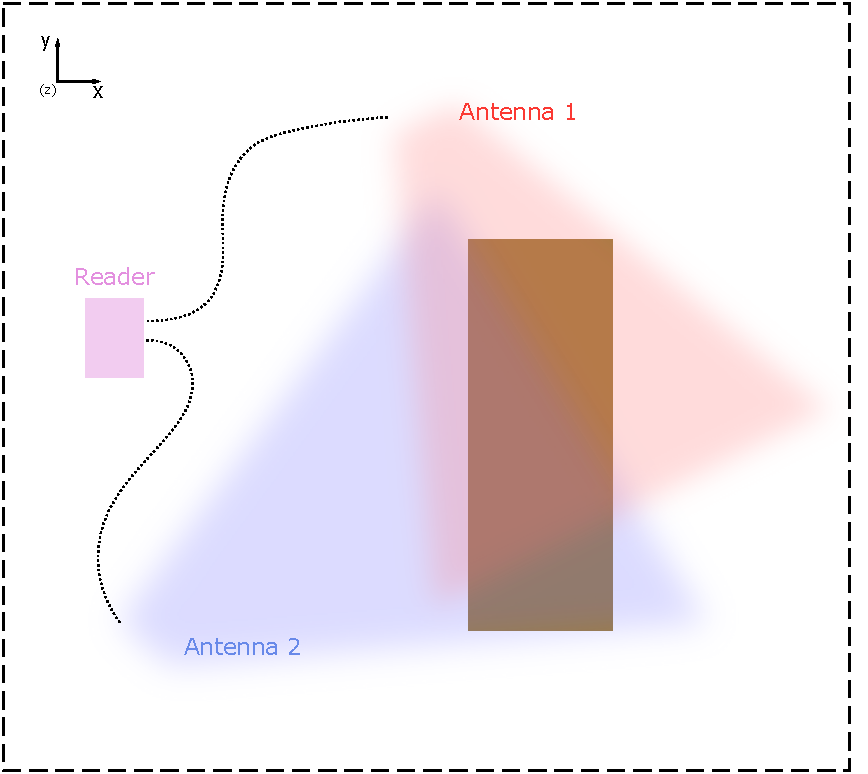
\includegraphics[width=0.5\linewidth]{./figs/02-state-of-the-art/position1.pdf}
    \caption{} 
    \label{fig:position1}
\end{figure}

Figures~\ref{fig:position21} and ~\ref{fig:position22} shows the most common approach to designing smart shelves, by placing one or multiple compact antennas in each shelve~\cite{markakisSafeEfficientDesign2014}.
These antennas can be incorporated into a shelf, making it invisible and ideal for point of sale and retail shelves.
Reading zones can be very precisely distributed, creating less \ac{rf} ``polution'', undesirable in contexts like shared warehouses in malls, where other \ac{rfid} system might be deployed.
The location techniques used in the first arrangement can be adapted and implemented in the same manner in this design.
This implementation has the downside of requiring multiple antennas, usually connected to reader will multiple antenna ports or to \ac{rf} splitters and multiplexers.

\begin{figure}[H]
    \centering
    \begin{subfigure}{.45\textwidth}
        \centering
        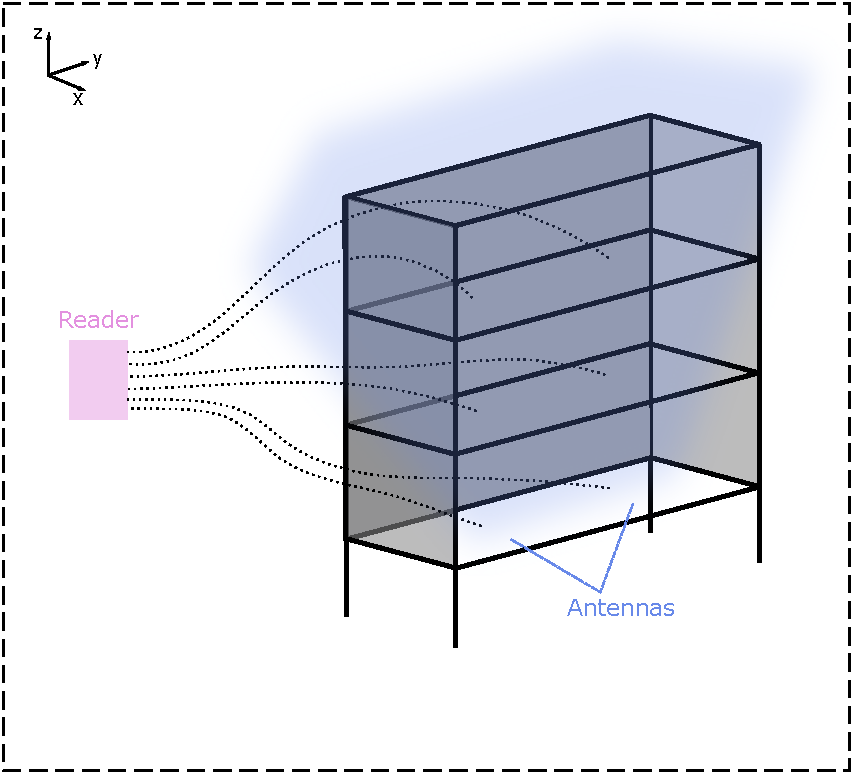
\includegraphics[width=\linewidth]{./figs/02-state-of-the-art/position2_1.pdf}
        \caption{} 
        \label{fig:position21}
    \end{subfigure}
    \begin{subfigure}{.45\textwidth}
        \centering
        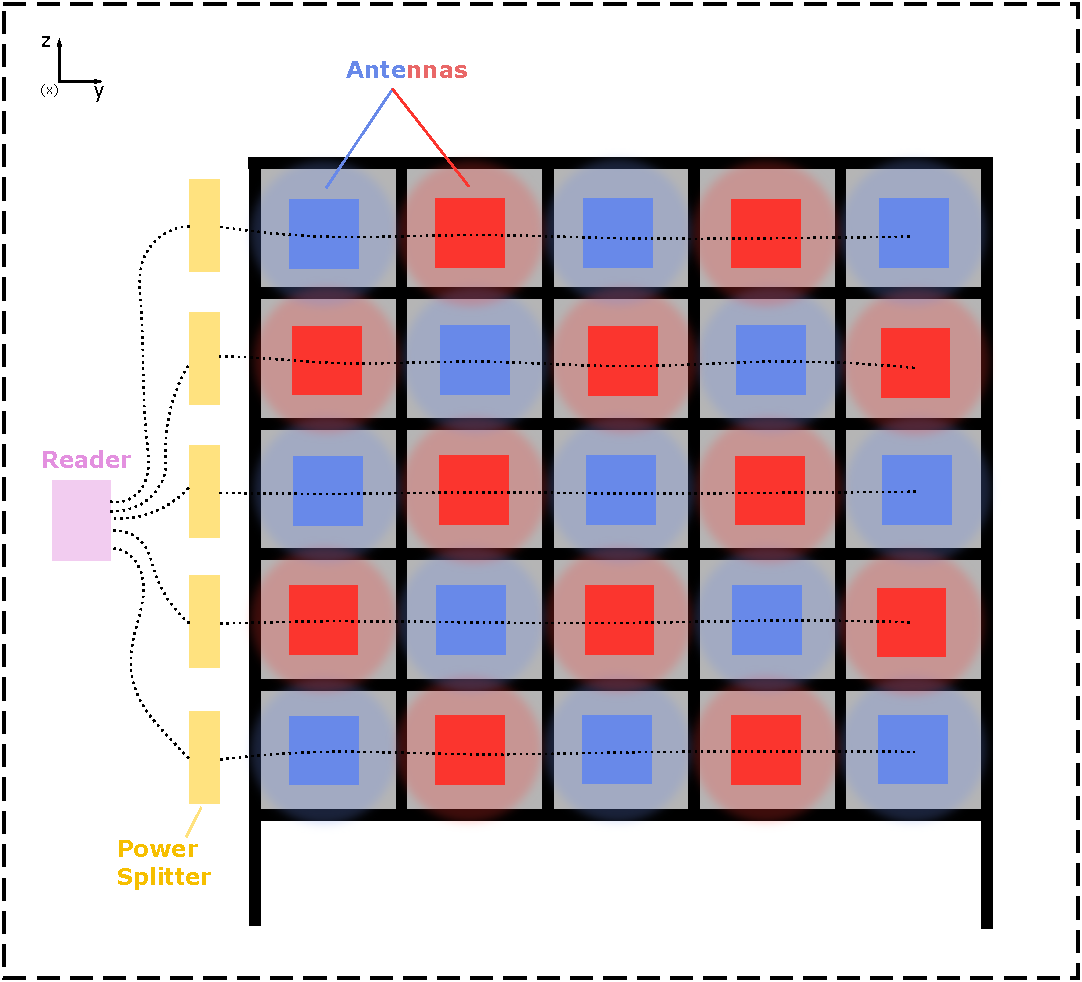
\includegraphics[width=\linewidth]{./figs/02-state-of-the-art/position2_2.pdf}
        \caption{} 
        \label{fig:position22}
    \end{subfigure}
    \caption{} 
    \label{fig:position2}
\end{figure}

The latest arrangement example, shown in figure~\ref{fig:position3}, places two antennas per shelf in the sides~\cite{markakisRFIDenabledLibraryManagement2013}. This approach can be implemented without the use of necessarily compact antennas and favors long shelf designs.
Opposite radiating angles can make location features a little tricky, regarding in shelf placement, whereby further study is needed.
Can be said that as downside of this arrangement is the necessity of multiple reader ports or \ac{rf} multiplexers, and in long shelves to have antenna designs tuned for both \emph{far} and \emph{near-fields}.

\begin{figure}[H]
    \centering
    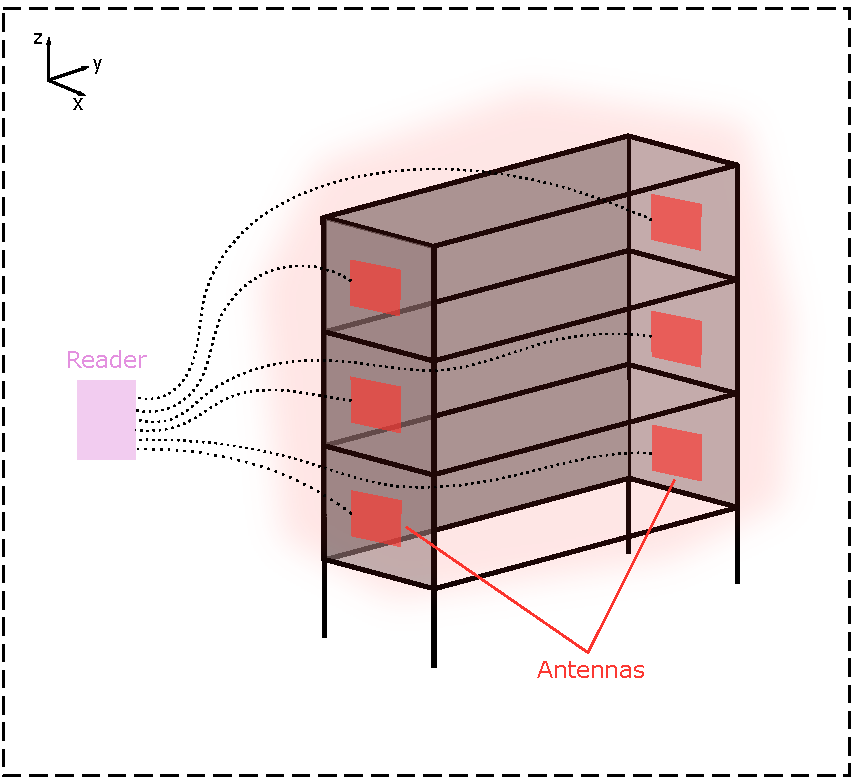
\includegraphics[width=0.5\linewidth]{./figs/02-state-of-the-art/position3.pdf}
    \caption{} 
    \label{fig:position3}
\end{figure}

\section{Software and Services}

This dissertation addresses two development ``timelines''. The first in which I evaluate the reader and shelve system: configure and test its capabilities, examine performance of the shelve system, interact with its interfaces. I also evaluate \ac{epc} encoding, decoding and translation software.
In the second period, the local deployment of the smart shelve system and \emph{EPCGlobal Architecture Framework} services.

For the first part, commercial readers manufacturers make Java and C# SDKs usually available. Readers providing an \ac{llrp} interface can also use \ac{llrp} client programs like the FossTrack LLRPCommander~\cite{FosstrakLLRPCommander}. There is also libraries available to decode and encode \ac{llrp} messages, which can be used to make \ac{llrp} clients. A few worth mention: Python \texttt{sllurp} and \texttt{pyllrp}, \ac{llrp} Toolkit Java, Perl and C\+\+ LTKs\cite{LlrpOrga}, Golang \texttt{go-llrp}).
To encode, decode and translate \acp{epc}, there are many available libraries, namely the \texttt{epc-standards} decoding Java library from Nike~\cite{NikeIncEpcstandards2019}, and Fosstrak Java \ac{tdt} Engine~\cite{FosstrakTagData}.

For the second part, the availability of resources is very limited.
The established software come from Fosstrak Open Source \ac{rfid} Software Platform, which provides a \ac{ale} \ac{fc} Middleware, Capturing Application and \ac{epcis} Repository. Fosstrack last commits to some projects are 5+ years old and the technology is outdated with bugs to the point that it can said it is broken, and the project forum is ``dead''.
Olliot is a fork of the Fosstrak components which extends GS1 standard architecture to support various \ac{iot} connectivity and protocols such as bar code, \ac{rfid} ZigBee and 6LoWPAN~\cite{OpenLanguageInternet}. Inherent to being based on Fosstrak code, it suffers, to certain degree, of the same problems as Fosstrak components.
Iori Mizutani, in this dissertation~\cite{mizutaniRobustHighPerformance} and research~\cite{mizutaniMulticodePortableRFID2016b}, has contributed with a modern implementaion in Golang of a \ac{fc} middleware and reader emulator~\cite{mizutaniIomzGolemu2020, mizutaniIomzGosstrak2020}. His work seems promising in the nonexistent contributions for the EPCGlobal standards in the last years. But his \ac{fc} implementation is not actively maintained anymore. It implements a simplified version of the \ac{ecspec} and provides a crude pseudo \ac{ale} interface, whereby not being production ready.

(commercial solutions)

Also worth mention, IoTA also supplies EPCGlobal tools in their ecosystem of distributed technology~\cite{GlobalTradeSupply}. It leverages on Fosstrak components to adds a prototype Discovery Service and secured \ac{epcis} components~\cite{FosstrakSimilarProjects}. Their platform of distributed network, block-chain, micropayments, immutable data and many other technologies reaches far out the scope of this dissertation.

\section{Out choice} \label{sec:ourchoice}
